\documentclass[a4paper]{article}
\usepackage[utf8]{vietnam}
\usepackage[left=3cm,right=2cm,top=2cm,bottom=2cm]{geometry}
\usepackage{amsmath}
\setlength{\parindent}{0pt}
\usepackage{graphicx} 
\usepackage{multirow}
\usepackage{url}
%\usepackage{wallpaper}
%\usepackage[firstpage]{draftwatermark} 
\usepackage{xcolor}
\usepackage{tikz} 
\usepackage{scrextend}
\usepackage{ulem}
\changefontsizes{13pt}
%\usepackage{background}
\usetikzlibrary{calc}
\usepackage{fancyhdr}
\usepackage[sorting=none]{biblatex}
\addbibresource{references.bib}

\usepackage{titlesec}
\usepackage{enumitem}
\usepackage{amsmath}
\titleformat{\section}{\fontsize{13}{15}\selectfont\bfseries}{\thesection}{1em}{}
\titleformat{\subsection}{\fontsize{13}{15}\selectfont\bfseries}{\thesubsection}{1em}{}
\usepackage{enumitem}
%----------------------- config của sy-------------
\usepackage{setspace}
\onehalfspacing
\usepackage{float}
\restylefloat{figure}
\floatplacement{figure}{H}
\usepackage{indentfirst}
\setlength{\parindent}{1cm}
%--------------------------------------Header footer------------------------------------
\pagestyle{fancy}
\fancyhf{} % Xóa định dạng hiện tại của header và footer

% Header
\lhead{Nhóm 2}
\chead{}
\rhead{Ứng dụng Kmeans phát hiện quả chín trong ảnh}

% Footer
\lfoot{}
\cfoot{} % Hiển thị số trang ở giữa footer
\rfoot{\thepage}

% Định dạng các đường line ở header và footer
\renewcommand{\headrulewidth}{0.1pt} % Độ dày của đường line ở header
\renewcommand{\footrulewidth}{0.1pt} % Độ dày của đường line ở footer
%---------------------------------------------------------------------------------------
%\backgroundsetup{scale = 1, angle = 0, opacity = 0.2,
%contents = {\includegraphics[width = 0.9\paperwidth,
%height = 0.9\paperheight, keepaspectratio] {hust.png}}}

%\backgroundsetup{scale = 1, angle = 0, opacity = 0.2,
%contents = {\includegraphics[width = 0.97\paperwidth,
%height = 0.97\paperheight, keepaspectratio] {bia.png}}}
\begin{document}

\begin{titlepage}
%\SetWatermarkText{\includegraphics[width = 0.97\paperwidth,
%height = 0.97\paperheight]{bia.png}}
%\SetWatermarkAngle{0} 
%\SetWatermarkText{\includegraphics[scale=1]{hust.png}}
%\SetWatermarkAngle{0} 
\begin{tikzpicture}[remember picture,overlay,inner sep=0,outer sep=0]
     \draw[black!80!black,line width=4pt] ([xshift=-2cm,yshift=-2cm]current page.north east) coordinate (A)--([xshift=3cm,yshift=-2cm]current page.north west) coordinate(B)--([xshift=3cm,yshift=2cm]current page.south west) coordinate (C)--([xshift=-2cm,yshift=2cm]current page.south east) coordinate(D)--cycle;

     \draw ([yshift=0.5cm,xshift=-0.5cm]A)-- ([yshift=0.5cm,xshift=0.5cm]B)--
     ([yshift=-0.5cm,xshift=0.5cm]B) --([yshift=-0.5cm,xshift=-0.5cm]B)--([yshift=0.5cm,xshift=-0.5cm]C)--([yshift=0.5cm,xshift=0.5cm]C)--([yshift=-0.5cm,xshift=0.5cm]C)-- ([yshift=-0.5cm,xshift=-0.5cm]D)--([yshift=0.5cm,xshift=-0.5cm]D)--([yshift=0.5cm,xshift=0.5cm]D)--([yshift=-0.5cm,xshift=0.5cm]A)--([yshift=-0.5cm,xshift=-0.5cm]A)--([yshift=0.5cm,xshift=-0.5cm]A);

     \draw ([yshift=-0.3cm,xshift=0.3cm]A)-- ([yshift=-0.3cm,xshift=-0.3cm]B)--
     ([yshift=0.3cm,xshift=-0.3cm]B) --([yshift=0.3cm,xshift=0.3cm]B)--([yshift=-0.3cm,xshift=0.3cm]C)--([yshift=-0.3cm,xshift=-0.3cm]C)--([yshift=0.3cm,xshift=-0.3cm]C)-- ([yshift=0.3cm,xshift=0.3cm]D)--([yshift=-0.3cm,xshift=0.3cm]D)--([yshift=-0.3cm,xshift=-0.3cm]D)--([yshift=0.3cm,xshift=-0.3cm]A)--([yshift=0.3cm,xshift=0.3cm]A)--([yshift=-0.3cm,xshift=0.3cm]A);

   \end{tikzpicture}


\begin{center}
    \vspace{7pt}
    \fontsize{14pt}{16pt}
    \textbf{TRƯỜNG ĐẠI HỌC BÁCH KHOA - ĐẠI HỌC ĐÀ NẴNG}
    
    \vspace{7pt}
    \textbf{KHOA ĐIỆN TỬ - VIỄN THÔNG} \\
    **************************
\end{center}
\vspace{10pt}
\begin{center}
    
\includegraphics[scale=0.37]{images/logodut.jpg}
    
\includegraphics[scale=0.75]{images/logoete.jpg}
    
    \vspace{20pt}
    \fontsize{20pt}{17pt}\selectfont 
    \textbf{BÁO CÁO} \\
    \vspace{7pt}
    \textbf{Học phần: Trí tuệ nhân tạo}
    \vspace{7pt}

\end{center}
\begin{flushleft}
    \fontsize{15pt}{10pt}\selectfont  
    \textbf{\textsl{\hspace{27pt}{\uline{ĐỀ TÀI:}}}}
\end{flushleft}
\begin{center}
    \hspace{10pt}
    \fontsize{17pt}{17pt}\selectfont 
    \textbf{\textrm{Ứng dụng KMeans phát hiện quả chín trong ảnh}}
\end{center}
\begin{center}
    \fontsize{16pt}{17pt}\selectfont 
    \textbf{\textrm{}}
\end{center}

\vspace{50pt}
\begin{addmargin}[1cm]{0cm}
\textbf{Giảng viên hướng dẫn: \hspace{2cm}Hoàng Lê Uyên Thục}
\end{addmargin}
\vspace{10pt}
% Bảng sinh viên thực hiện thụt vào 2cm
\begin{addmargin}[1cm]{0cm}
\textbf{Sinh viên thực hiện: \hspace{2.6cm}NHÓM 2}
\begin{tabbing}
\hspace{4cm}\=\hspace{3cm}\=\hspace{5cm} \kill
{\textbf{Họ và tên}}\>{\textbf{MSSV}}\>{\textbf{Email liên hệ}}\\
\hspace{4cm}\=\hspace{3cm}\=\hspace{5cm} \kill
Lê Phạm Công\> 106200221\> lpc051002@gmail.com\\
\hspace{4cm}\=\hspace{3cm}\=\hspace{5cm} \kill
Phan Công Danh\> 106200222\> phancongdanh1542k2@gmail.com\\
\hspace{4cm}\=\hspace{3cm}\=\hspace{5cm} \kill
Đoàn Thế Lên\> 106200233\> lendoan07@gmail.com\\
\hspace{4cm}\=\hspace{3cm}\=\hspace{5cm} \kill
Lê Minh Nhật\> 106200238\> minhat13579@gmail.com\\
\end{tabbing}
\end{addmargin}
\vspace{1cm}
\begin{center}
    \textit{\textbf{Đà Nẵng, ngày 13 tháng 05 năm 2024}}
\end{center}
\end{titlepage}
% -------------------------------------End trang bìa-----------------------
\newpage
\tableofcontents
\newpage

% ----------------------- MAIN DOCUMENT---------------------------%

\section*{Tóm tắt}
\addcontentsline{toc}{section}{Tóm tắt}
Trong báo cáo này trình bày một giải pháp hiệu quả sử dụng thuật toán phân cụm K-means++ để phân đoạn và phát hiện các quả chín trong ảnh. Trong phương pháp đề xuất, ảnh đầu vào được biến đổi sang không gian màu thích hợp, sau đó áp dụng thuật toán K-means++ để phân cụm các điểm ảnh dựa trên đặc trưng màu sắc và vị trí. Các điểm ảnh thuộc cùng một cụm được xem là đại diện cho một đối tượng trong ảnh. Bằng cách phân tích màu sắc của quả chín sau khi phân cụm, các quả chín có thể được phát hiện và đánh dấu trên ảnh. Kết quả thực nghiệm cho thấy phương pháp đề xuất đạt hiệu suất tốt trong việc phát hiện các quả chín. Phương pháp này có thể được ứng dụng trong các hệ thống nông nghiệp thông minh và nhiều ứng dụng trong tương lai.

Mã nguồn của báo cáo có thể được tìm thấy tại \url{https://github.com/lephamcong/KMeans_Detect_Ripe_Fruit.git}

\section{Giới thiệu}
Trong ngành nông nghiệp hiện đại, việc tự động hóa quá trình thu hoạch không chỉ giúp tăng hiệu quả sản xuất mà còn giảm thiểu đáng kể chi phí lao động và thời gian. Một trong những khó khăn chính trong tự động hóa này là khả năng xác định và phân loại quả chín từ quả chưa chín qua hình ảnh, một nhiệm vụ quan trọng trong quyết định thời điểm thu hoạch. Nhận diện quả chín chính xác thông qua hệ thống máy tính cung cấp một giải pháp tiềm năng để tối ưu hóa quy trình thu hoạch và giảm thiểu tổn thất sau thu hoạch.

Thuật toán KMeans, một kỹ thuật phân cụm dữ liệu không giám sát, đã được chứng minh là có hiệu quả trong nhiều lĩnh vực phân tích ảnh do khả năng phân loại dữ liệu dựa trên các tính năng được trích xuất. Báo cáo này khám phá việc ứng dụng thuật toán Kmeans để phát hiện chín trong các bức ảnh chụp và đề xuất phương pháp với ứng dụng của thuật toán Kmeans có thể phân biệt quả chín với quả chưa chín dựa trên màu sắc, đây là đặc điểm dễ quan sát nhất và có ảnh hưởng lớn đến quyết định thu hoạch của hầu hết các loại trái cây.

\section{Phương pháp}
Thuật toán phân cụm KMeans là một trong những thuật toán phân cụm dữ liệu đơn giản dựa trên học không giám sát (Unsupervised learning). Unsupervised learning, hay học không giám sát, là một nhánh của học máy trong đó mô hình được huấn luyện từ dữ liệu không có nhãn. Điều này có nghĩa là trong quá trình huấn luyện, dữ liệu đầu vào không đi kèm với đầu ra mong muốn. Mục tiêu của học không giám sát là khám phá cấu trúc ẩn và các mối liên hệ trong dữ liệu không được gán nhãn.

\subsection{Thuật toán KMeans và KMeans++}
Thuật toán phân cụm K-means được giới thiệu năm 1957 bởi Lloyd K-means và là phương pháp phổ biến nhất cho việc phân cụm, dựa trên việc phân vùng dữ liệu.

Biểu diễn dữ liệu $D={x_1, x_2, x_3, \dots, x_i}$, với $x_i$ là vector n chiều trong không gian Euclidean. K-means phân cụm D thành K cụm dữ liệu:
\begin{itemize}
    \item Mỗi cụm dữ liệu có một điểm trung tâm gọi là centroid.
    \item K là một hằng số cho trước, là số cluster cần phân cụm. 
\end{itemize}
Mục tiêu của thuật toán KMeans là phân chia n dữ liệu thành K cụm (clusters) dựa trên các đặc điểm của dữ liệu, sao cho dữ liệu trong cùng một cụm có sự tương đồng cao với nhau và có sự
khác biệt với dữ liệu trong các cụm khác.Ý tưởng đơn giản nhất về cluster (cụm) là tập hợp các điểm ở gần nhau trong một không gian nào đó (không gian này có thể có rất nhiều chiều trong trường hợp thông tin về một điểm dữ liệu là rất lớn). Hình \ref{fig:3_cluster} là một ví dụ về 3 cụm dữ liệu (cluster), mỗi cluster tương ứng với 1 màu và các centroid màu vàng tương ứng với từng cluster.

\begin{figure}[h] 
    \centering 
    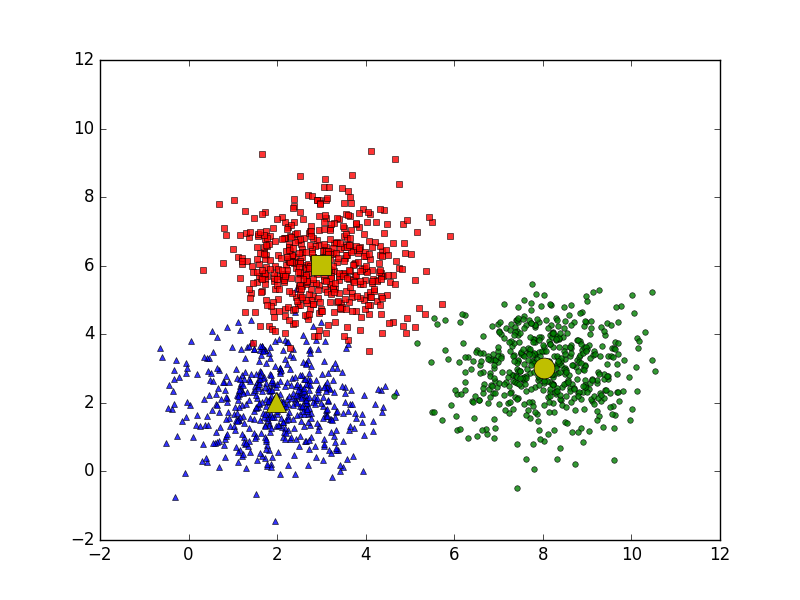
\includegraphics[width=1\textwidth]{images/3_cluster.png} 
    \textit{\caption{Ví dụ về dữ liệu được phân thành 3 cụm}}
    \label{fig:3_cluster} 
\end{figure}
\textbf{Các bước trong thuật toán KMeans\cite{KMeansCluster}:}
\begin{itemize}[label={}]
    \item \textbf{Đầu vào:} Cho tập dữ liệu D, với K là số cụm, phép đo khoảng cách giữa 2 điểm dữ liệu là d(x,y)
    \item \textbf{Khởi tạo:} Khởi tạo K điểm dữ liệu trong D làm các điểm trung tâm (centroid)
    \item  \textbf{Lặp lại các bước sau đến khi hội tụ:}
    \begin{itemize}[label={}]
        \item  \textbf{Bước 1:} Với mỗi điểm dữ liệu, gán điểm dữ liệu đó vào cluster có khoảng cách đến điểm trung tâm của cluster là nhỏ nhất.
        \item  \textbf{Bước 2:} Với mỗi cluster, xác định lại điểm trung tâm của tất cả các điểm dữ liệu được gán vào cluster đó.
    \end{itemize}
    \item \textbf{Đầu ra:} Các centroid M và label vector cho từng điểm dữ liệu Y
\end{itemize}

Hình \ref{fig:interation1} mô tả quá trình khởi tạo K điểm dữ liệu trong D làm các centroid. Sau đó gán các điểm dữ liệu vào các cluster có khoảng cách đến centroid là nhỏ nhất (B), tiếp theo tính toán lại centroid của cluster và tiến hành phân cụm lại dựa trên các centroid mới (C).
\begin{figure}[h] 
    \centering 
    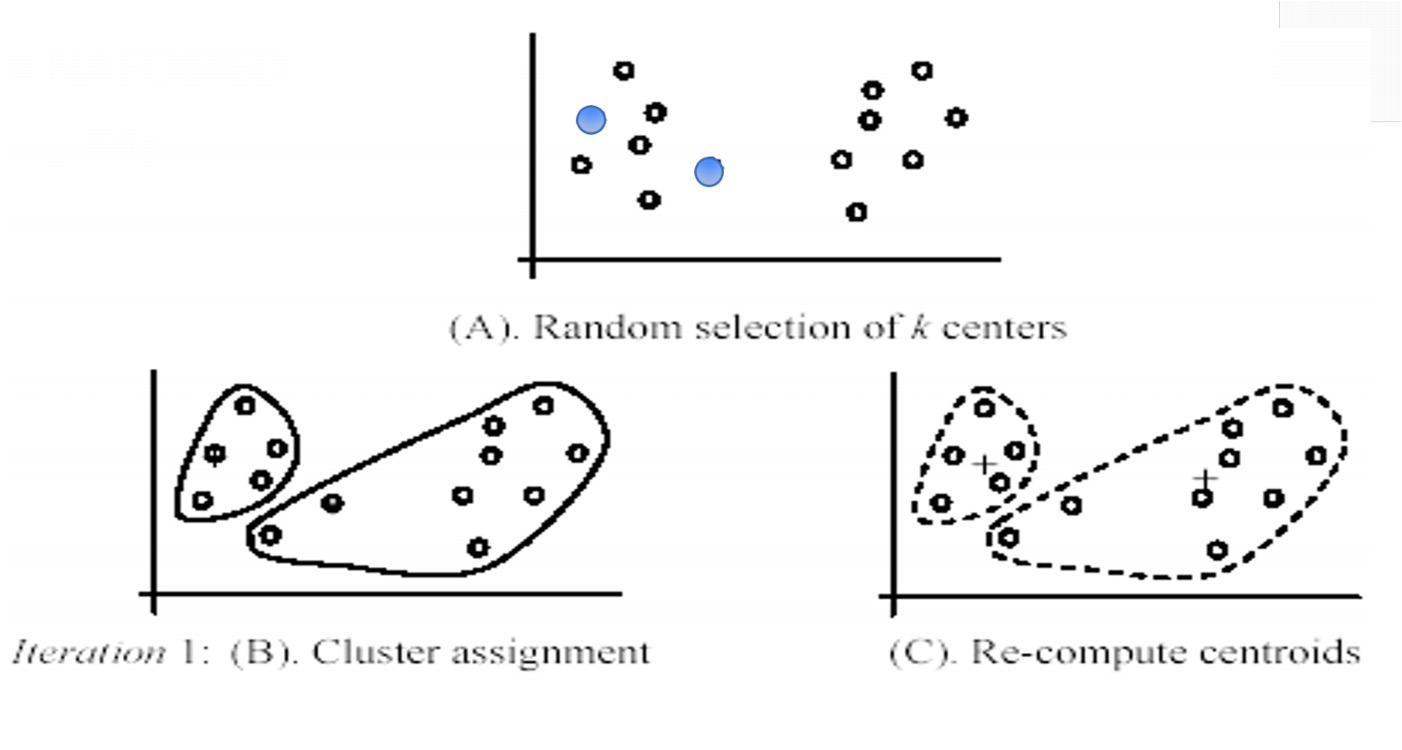
\includegraphics[width=0.9\textwidth]{images/interation1.png} 
    \textit{\caption{Khởi tạo K cụm ngẫu nhiên và tính toán centroid cho các cụm \cite{KMeansCluster}}} 
    \label{fig:interation1} 
\end{figure}

Hình \ref{fig:interation2-3} mô quá trình lặp lại các bước tính toán như hình \ref{fig:interation1} cho đến khi hội tụ thì dừng quá trình phân cụm.
\begin{figure}[h] 
    \centering 
    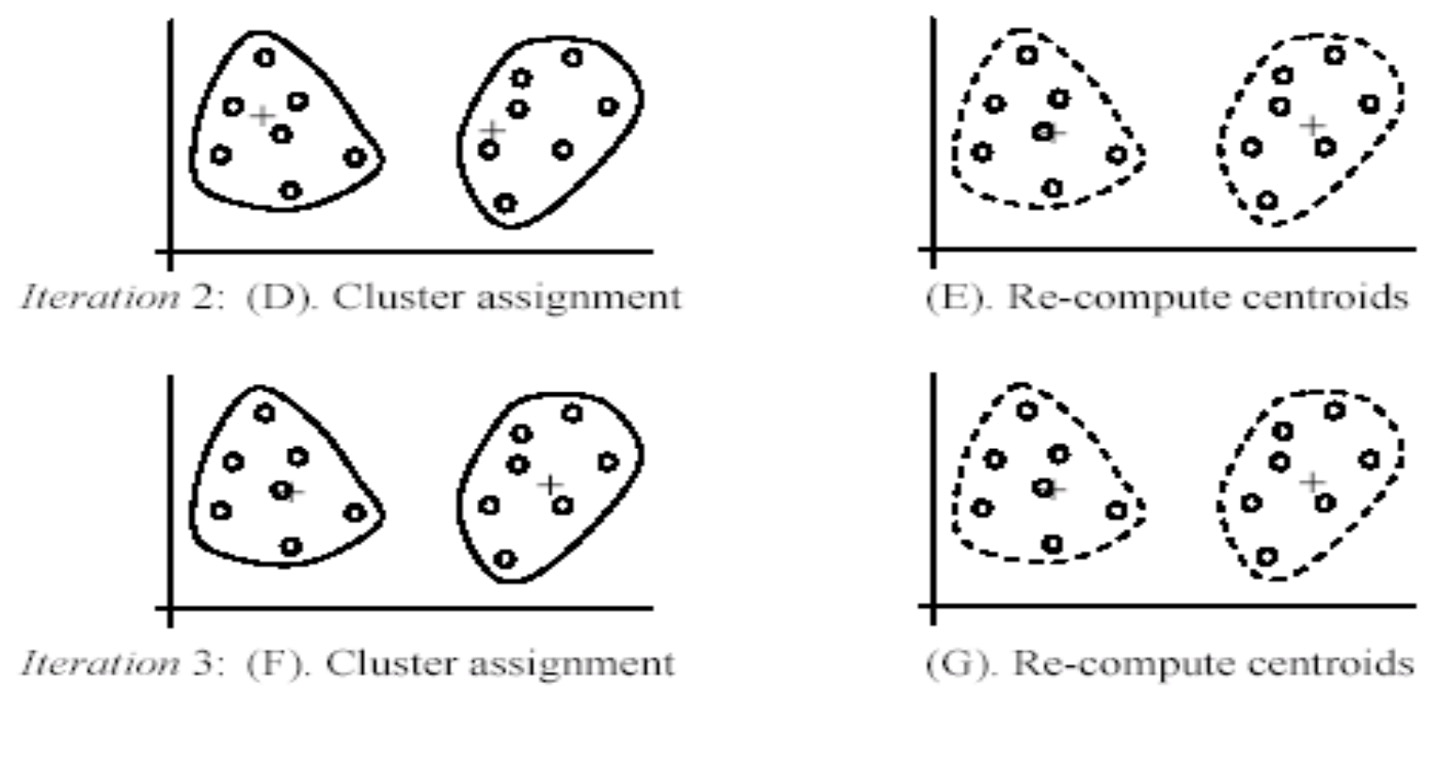
\includegraphics[width=0.85\textwidth]{images/interation2-3.png} 
    \textit{\caption{Quá trình tính toán các centroid cho đến khi hội tụ \cite{KMeansCluster}}}
    \label{fig:interation2-3} 
\end{figure}

\textbf{Điều kiện hội tụ (điều kiện dừng thuật toán)\cite{KMeansCluster}}
Có thể sử dụng các điều kiện sau là điều kiện hội tụ:
\begin{itemize}[label={}]
    \item \textbf{1. }Tại 1 vòng lặp: có ít các điểm dữ liệu được gán sang cluster khác hoặc
    \item \textbf{2. }Điểm trung tâm (centroid) không thay đổi nhiều hoặc
    \item \textbf{3. }Giá trị hàm mất mát (công thức \ref{eq:loss_function}) không thay đổi nhiều:
    \begin{equation}
        \text{Error} = \sum_{i=1}^{k} \sum_{x \in C_i} d(x, m_i)^2
        \label{eq:loss_function}
    \end{equation}
    Trong đó: $C_i$ là cluster thứ i, $m_i$  là điểm trung tâm của cluster $C_i$ tương ứng. \\
    Nhìn chung về điều kiện hội tụ có thể thấy mối liên hệ giữa các điều kiện là gần tương đồng như nhau. Khi có ít điểm dữ liệu được gán sang cluster khác có thể khiến điểm trung tâm không thay đổi nhiều và từ đó hàm mất mát cũng sẽ ít bị ảnh hưởng. Vậy nên có thể sử dụng 1 trong 3 cách trên để xác định điều kiện dừng của thuật toán
\end{itemize}
Trong K-means để đánh giá mức độ giống nhau hay khoảng cách giữa 2 điểm dữ liệu có thể sử dụng các phép đo khoảng cách khác nhau. Ngoài khoảng cách Euclidean, tuỳ thuộc vào từng bài toán có thể sử dụng phương pháp đo khác (cosine, manhattan…). Khoảng cách Euclidean được tính bằng cách lấy căn bậc hai của tổng bình phương các hiệu giữa tọa độ tương ứng của hai điểm trong không gian nhiều chiều.

Công thức cho khoảng cách Euclidean giữa hai điểm x và $m_i$ trong không gian n-chiều là:
\begin{equation}
    d(x, m_i) = \|\mathbf{x} - \mathbf{m}_i\| = \sqrt{(x_1 - m_{i1})^2 + (x_2 - m_{i2})^2 + \ldots + (x_n - m_{in})^2}
    \label{eq:euclidean}
\end{equation}
Trong đó \( x = (x_1, x_2, \ldots, x_n) \) và \( m_i = (m_{i1}, m_{i2}, \ldots, m_{in}) \) là các vector trong không gian n-chiều, biểu diễn tọa độ của hai điểm. Phép đo này thường được sử dụng trong nhiều thuật toán học máy và phân tích dữ liệu, đặc biệt là trong các thuật toán phân cụm như K-means, vì nó đo lường trực tiếp khoảng cách "thẳng" giữa hai điểm trong không gian nhiều chiều.

Một hạn chế của thuật toán KMeans là sự phụ thuộc cao vào việc khởi tạo các centroid. Nếu một centroid được khởi tạo ở vị trí quá xa, có thể nó sẽ không có điểm dữ liệu nào được gán vào nó, khiến cho centroid đó vô nghĩa. Đồng thời, điều này cũng có thể dẫn đến việc nhiều cụm có chung một centroid. Tương tự, việc khởi tạo nhiều centroid trong cùng một cụm có thể gây ra phân cụm không hiệu quả. Để giải quyết vấn đề này, giải pháp được sử dụng trong nghiên cứu này là thay thế việc sử dụng KMeans truyền thống bằng KMeans++\cite{GeeksForGeeksKMeans}. Quá trình khởi tạo các centroid trong KMeans++:
\begin{itemize}[label={}]
    \item \textbf{Bước 1: }Chọn ngẫu nhiên trọng tâm đầu tiên từ các điểm dữ liệu.
    \item \textbf{Bước 2: }Đối với mỗi điểm dữ liệu, tính khoảng cách của nó đến trọng tâm đã chọn gần nhất trước đó.
    \item \textbf{Bước 3: }Chọn trọng tâm tiếp theo từ các điểm dữ liệu sao cho xác suất chọn một điểm làm trọng tâm tỷ lệ thuận với khoảng cách của nó đến trọng tâm đã chọn gần nhất trước đó (tức là điểm có khoảng cách xa nhất từ trọng tâm gần nhất sẽ có khả năng cao được chọn làm trọng tâm tiếp theo).
    \item \textbf{Bước 4: }Lặp lại các bước 2 và 3 cho đến khi đã chọn được k trọng tâm.
\end{itemize}


Thuật toán KMeans++ cải tiến cách khởi tạo các centroid, từ đó nâng cao chất lượng phân cụm. Trừ bước khởi tạo, các bước còn lại của thuật toán này hoàn toàn tương tự như thuật toán KMeans truyền thống. Có thể nói, KMeans++ chính là thuật toán KMeans được bổ sung thêm phần khởi tạo centroid một cách thông minh hơn. Mặc dù việc khởi tạo trong K-means++ tốn kém hơn về mặt tính toán so với thuật toán K-means tiêu chuẩn, thời gian chạy để hội tụ đến giải pháp tối ưu lại được giảm đáng kể cho K-means++. Điều này là bởi vì các trọng tâm được chọn ban đầu có khả năng nằm trong các cụm khác nhau ngay từ đầu.
\newpage
\subsection{Phát hiện quả chín trong ảnh}

\begin{figure}[h] 
    \centering 
    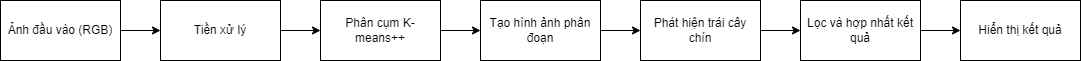
\includegraphics[width=0.85\textwidth]{images/sodohethong.png} 
    \textit{\caption{Sơ đồ hệ thống phát hiện quả chín trong ảnh}}
    \label{fig:sodohethong} 
\end{figure}

Hình 4 biểu diễn quy trình xử lý hình ảnh để phát hiện trái cây chín trong một hệ thống tự động dựa trên thuật toán K-means++:
\begin{itemize}[label={}]
    \item \textbf{Giai đoạn 1. Ảnh đầu vào (RGB):} 
    \begin{itemize}[label={}]
        \item \textbf{Nguồn dữ liệu:} Hình ảnh có thể được nhập từ nhiều nguồn như tệp lưu trữ, camera trực tiếp, hoặc thư viện hình ảnh. 
        \item  \textbf{Định dạng đầu vào:} Hình ảnh có thể ở các định dạng khác nhau như JPEG, PNG, hoặc BMP. Cần phải xử lý để chuyển đổi thành định dạng phù hợp cho việc xử lý tiếp theo.
    \end{itemize}
    \item \textbf{Giai đoạn 2. Tiền xử lý: }
    \begin{itemize}[label={}]
        \item \textbf{Chuyển đổi không gian màu:} Chuyển đổi hình ảnh từ không gian màu BGR (mặc định của OpenCV) sang RGB để phù hợp với các chuẩn xử lý hình ảnh thường dùng trong phân tích và xử lý.
        \item \textbf{Chuẩn hóa dữ liệu:} Điều chỉnh kích thước hình ảnh nếu cần để đồng bộ hóa quy trình xử lý, hoặc áp dụng các bước tiền xử lý khác như làm mịn để giảm nhiễu.
    \end{itemize}
    \item  \textbf{Giai đoạn 3. Phân cụm K-means++: }
    \begin{itemize}[label={}]
        \item \textbf{Chuyển đổi dữ liệu:} Chuyển hình ảnh đã được tiền xử lý thành một mảng 2D của pixel để dễ dàng xử lý trong thuật toán phân cụm.
        \item \textbf{Áp dụng thuật toán K-means++:} Sử dụng thuật toán K-means++ để phân chia các pixel thành các nhóm dựa trên sự giống nhau về màu sắc, sử dụng phương pháp khởi tạo thông minh để cải thiện hiệu quả phân cụm.
        \item \textbf{Thuật toán Kmeans++ được sử dụng có thể giải thích như sau: }
        \begin{itemize}[label={}]
            \item \textbf{Bước 1. }Khởi tạo centroid đầu tiên một cách ngẫu nhiên: Chọn ngẫu nhiên một số K điểm dữ liệu để làm các centroid ban đầu cho K cụm.
            \item \textbf{Bước 2. }Lặp lại cho mỗi centroid còn lại (sau khi đã có centroid đầu tiên):
            \begin{itemize}[label={}]
                \item Tính khoảng cách từ centroid này tới các centroid hiện có.
                \item Xác định xác suất chọn mỗi điểm dữ liệu dựa trên khoảng cách đó (các điểm xa hơn có xác suất thấp hơn).
                \item Chọn ngẫu nhiên một điểm dữ liệu làm centroid mới dựa trên xác suất đó.
            \end{itemize}
            \item \textbf{Bước 3. }Lặp lại cho đến khi đạt số vòng lặp tối đa hoặc thuật toán hội tụ:
            \begin{itemize}[label={}]
                \item Gán mỗi điểm dữ liệu vào cụm có centroid gần nhất.
                \item Tính lại vị trí các centroid dựa trên trung bình của các điểm trong cụm đó.
                \item Kiểm tra điều kiện hội tụ (ví dụ không có sự thay đổi nào trong việc gán cụm).
            \end{itemize}
            \item \textbf{Bước 4. }Trả về kết quả là các điểm dữ liệu được gán cho từng cụm và vị trí của các centroid cuối cùng.
        \end{itemize}
    \end{itemize} 
    \item \textbf{Giai đoạn 4. Tạo hình ảnh phân đoạn:} Mỗi pixel được ánh xạ tới trung tâm cụm tương ứng, tạo ra một hình ảnh phân đoạn mà mỗi khu vực màu sắc đại diện cho một cụm.
    \item \textbf{Giai đoạn 5. Phát hiện trái cây chín:}
    \begin{itemize}[label={}]
        \item \textbf{Áp dụng ngưỡng màu:} Thiết lập một ngưỡng màu để phát hiện các vùng màu đỏ, phù hợp với màu của trái cây chín trong hình ảnh.
        \item \textbf{Xác định vị trí trái cây:} Sử dụng các kỹ thuật xử lý hình ảnh như tìm đường viền để xác định vị trí của trái cây trong hình ảnh.
    \end{itemize}
    \item \textbf{Giai đoạn 6. Lọc và hợp nhất kết quả:}
    \begin{itemize}[label={}]
        \item \textbf{Xử lý các đối tượng nhỏ:} Loại bỏ các đối tượng nhỏ không đáng kể để giảm nhiễu và sai số.
        \item \textbf{Xử lý các đối tượng gần nhau:} Hợp nhất các đối tượng lân cận để tạo thành một hình ảnh rõ ràng và dễ phân tích hơn.
    \end{itemize}
    \item \textbf{Giai đoạn 7. Hiển thị kết quả}
    \begin{itemize}[label={}]
        \item \textbf{Vẽ hộp giới hạn:} Dùng các hộp giới hạn màu để đánh dấu các trái cây chín trên hình ảnh.
        \item \textbf{Nhãn dán:} Gán nhãn cho các trái cây để dễ dàng nhận biết.
    \end{itemize}
\end{itemize}
\newpage
\section{Thực hiện}
\begin{itemize}[label={}]
    \item Ngôn ngữ lập trình: Python 3.11.2
    \item Các thư viện sử dụng:
    \begin{itemize}[label={}]
        \item opencv-python==4.9.0.80
        \item numpy==1.26.4
        \item matplotlib==3.7.1
        \item pkg-resources==None
    \end{itemize}
    \item Dataset: \url{https://drive.google.com/drive/folders/1GwVZU8G0OG5C4-ou9f9QJ62rsi_Dmi_6?usp=sharing}
\end{itemize}
\subsection{Kết quả}
Dưới đây là một số kết quả thu được khi thử nghiệm với tập dữ liệu là ảnh quả chín (gồm 2 trường hợp là ảnh 1 quả chín và ảnh nhiều quả chín), ảnh kết quả bao gồm ảnh gốc (bên trái) và ảnh đã phát hiện quả chín (bên phải):
\begin{figure}[h] 
    \centering 
    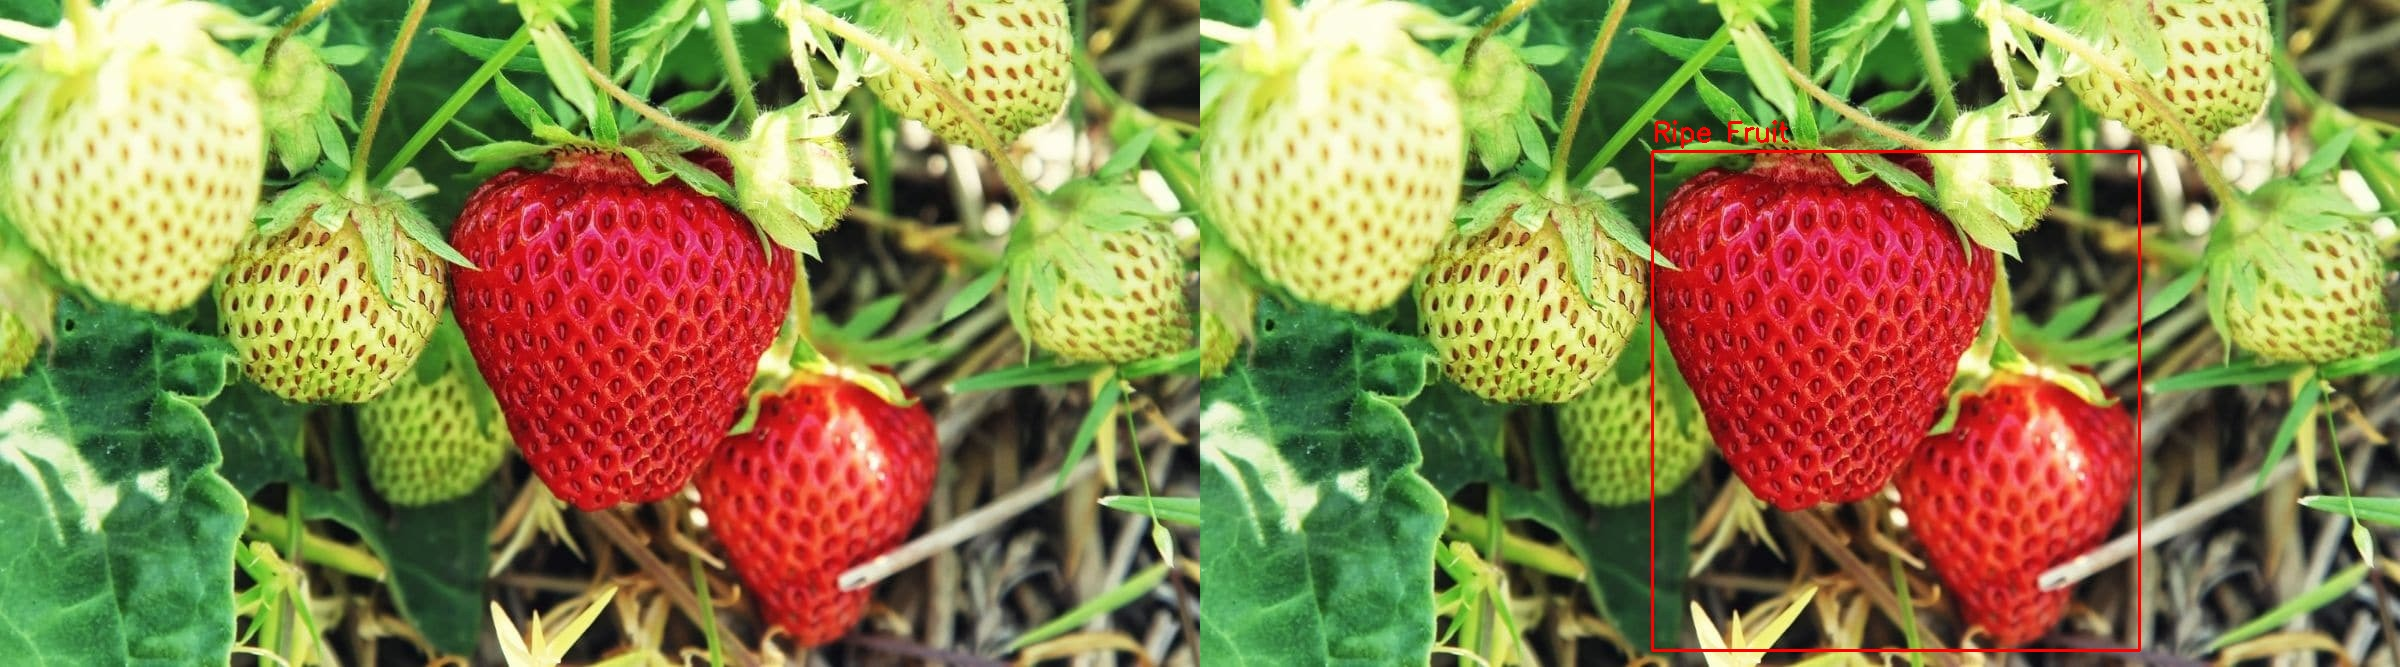
\includegraphics[width=0.8\textwidth]{images/result/ripe1.jpg} 
    \textit{\caption{Kết quả 1}}
    \label{fig:ketqua1} 
\end{figure}
\begin{figure}[h] 
    \centering 
    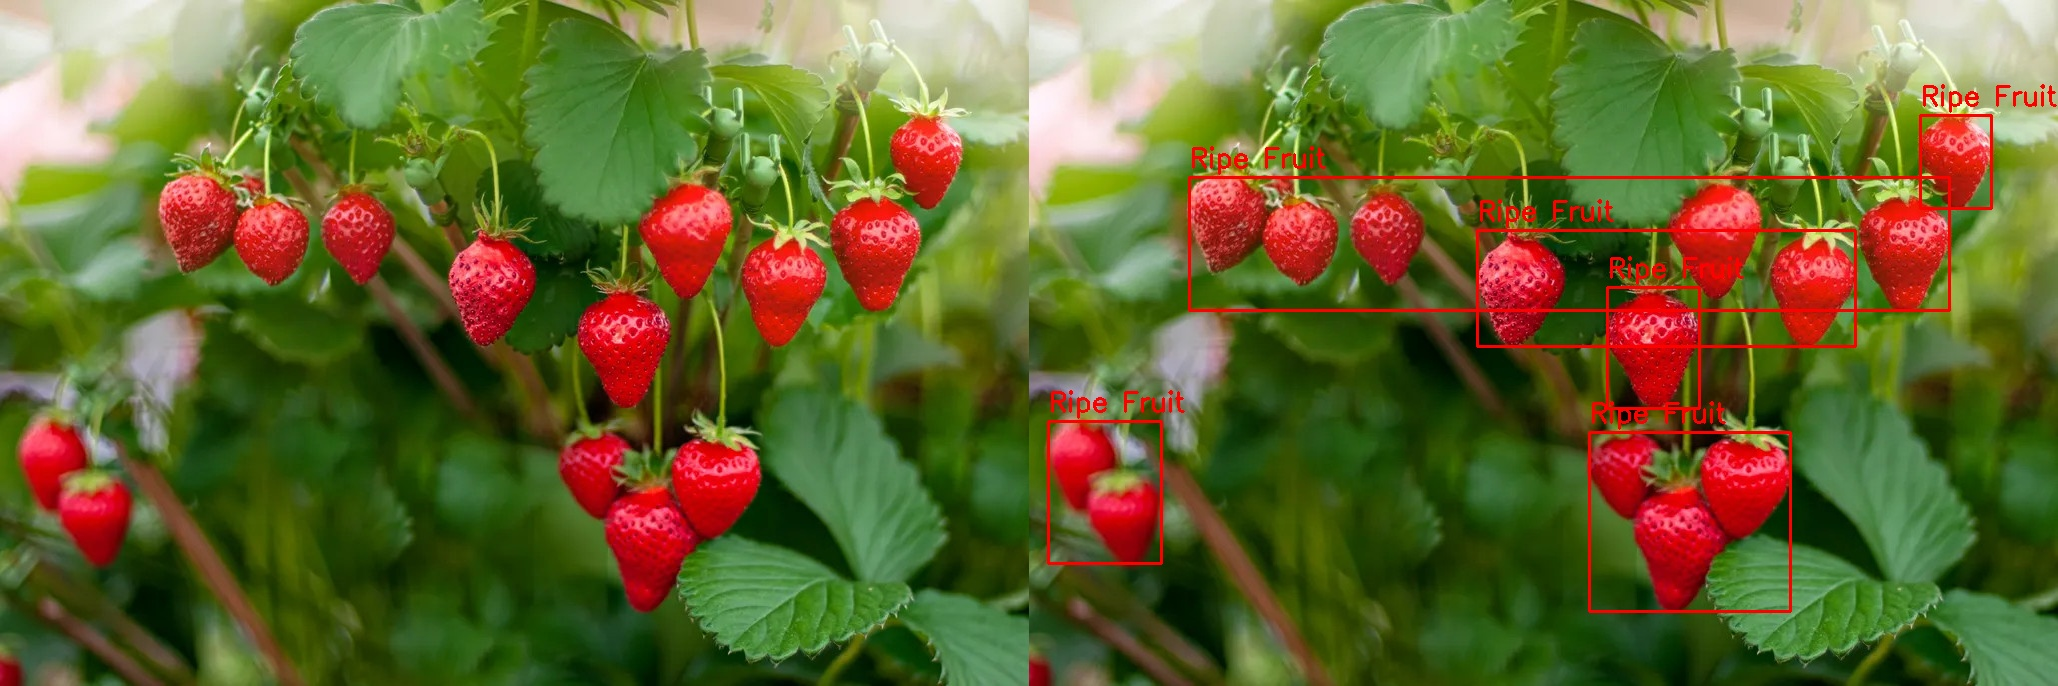
\includegraphics[width=0.8\textwidth]{images/result/ripe2.jpg} 
    \textit{\caption{Kết quả 2}}
    \label{fig:ketqua2} 
\end{figure}
\begin{figure}[h] 
    \centering 
    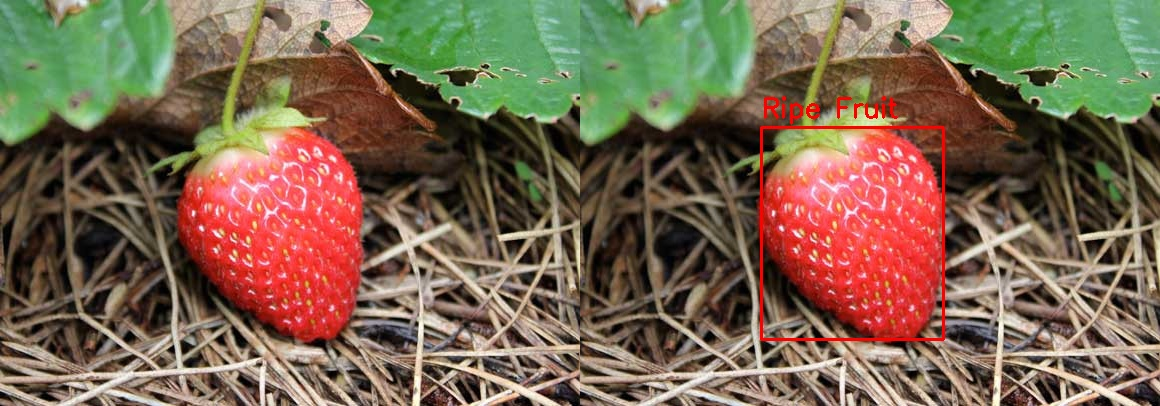
\includegraphics[width=0.8\textwidth]{images/result/ripe3.jpg} 
    \textit{\caption{Kết quả 3}}
    \label{fig:ketqua3} 
\end{figure}
\begin{figure}[h] 
    \centering 
    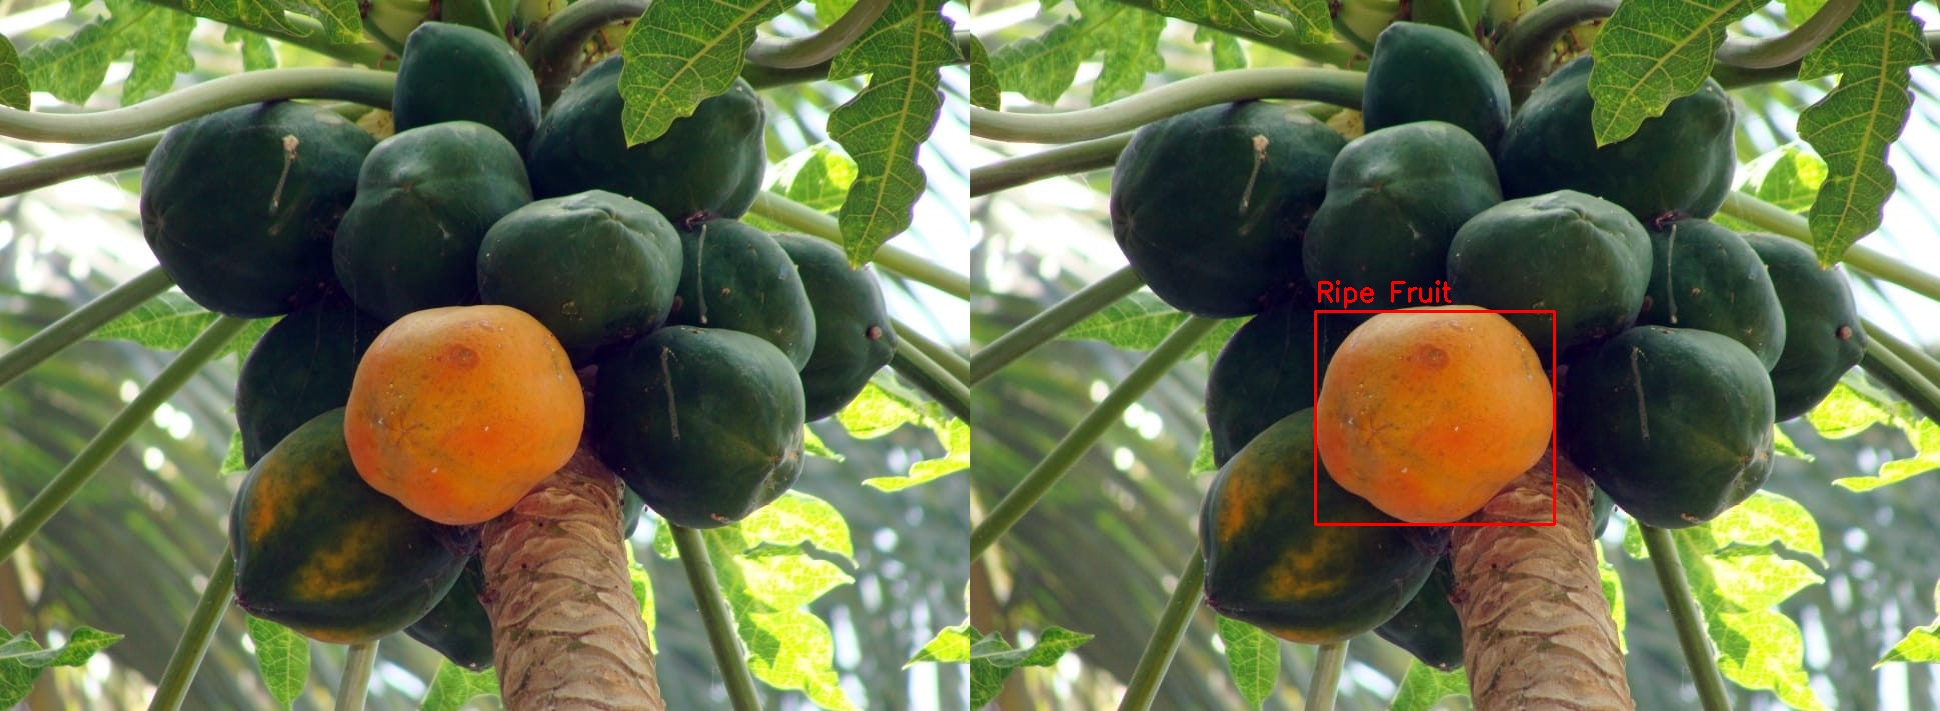
\includegraphics[width=0.8\textwidth]{images/result/ripe4.jpg} 
    \textit{\caption{Kết quả 4}}
    \label{fig:ketqua4} 
\end{figure}

\newpage
\subsection{Đánh giá}
Việc sử dụng thuật toán KMeans, đặc biệt là phiên bản KMeans++ để phát hiện quả chín trong ảnh có những ưu điểm và hạn chế nhất định: \\
\textbf{Ưu điểm:} \\
\textit{Đơn giản và hiệu quả:} Thuật toán KMeans++ khá đơn giản và dễ triển khai. Nó hoạt động hiệu quả trong việc phân cụm dữ liệu dựa trên đặc trưng màu sắc và vị trí. \\
\textit{Khả năng xử lý dữ liệu lớn:} KMeans++ có thể xử lý các tập dữ liệu ảnh lớn với số lượng điểm ảnh nhiều mà không bị ảnh hưởng đáng kể về hiệu suất. \\
\textit{Không giám sát: }KMeans++ là một thuật toán phân cụm không giám sát, không yêu cầu dữ liệu đã được gán nhãn trước, phù hợp với bài toán phát hiện quả chín.\\ 
\textit{Tính linh hoạt:} Có thể điều chỉnh số lượng cụm K để phù hợp với các loại quả khác nhau hoặc điều kiện môi trường khác nhau. \\
\textbf{Hạn chế:} \\
\textit{Nhạy cảm với nhiễu và giá trị ngoại lai:} Thuật toán KMeans++ có thể bị ảnh hưởng bởi nhiễu trong ảnh hoặc các giá trị ngoại lai, dẫn đến kết quả phân cụm không chính xác. \\
\textit{Khó xác định số lượng cụm tối ưu:} Việc lựa chọn số lượng cụm K phù hợp là một thách thức, và có thể ảnh hưởng đến kết quả phân cụm. \\
\textit{Không phù hợp với cụm có hình dạng phức tạp:} KMeans++ hoạt động tốt nhất với các cụm có hình dạng gần đúng hình cầu. Đối với các cụm có hình dạng phức tạp, hiệu suất có thể giảm.
Khó phát hiện các quả chín có màu sắc tương tự với nền: Nếu màu sắc của quả chín quá tương tự với màu nền trong ảnh, thuật toán có thể gặp khó khăn trong việc phân biệt chúng. 

Để giải quyết các hạn chế trên, có thể kết hợp KMeans++ với các kỹ thuật xử lý ảnh khác như tách nền, làm mịn ảnh, hoặc sử dụng các đặc trưng bổ sung như hình dạng, kích thước để cải thiện hiệu suất phát hiện quả chín. Ngoài ra, các phương pháp phân cụm khác như phân cụm mật độ, phân cụm phân cực có thể được xem xét để xử lý các trường hợp phức tạp hơn.

\section{Kết luận}
Trong bài toán phát hiện quả chín trong ảnh, KMeans có thể được áp dụng để
phân cụm các điểm ảnh dựa trên màu sắc, kết cấu hoặc đặc trưng khác của quả. Tuy
nhiên, để đạt được kết quả tốt hơn, cần kết hợp KMeans với các kỹ thuật xử lý ảnh
khác như phân tích hình dạng, kết cấu, ...

Đối với bài toán phát hiện đối tượng nói chung, KMeans có thể được sử dụng như
một bước tiền xử lý để phân cụm dữ liệu ảnh hoặc dữ liệu đa chiều khác, giúp giảm
kích thước dữ liệu và tăng hiệu suất của các thuật toán phát hiện đối tượng phức tạp
hơn. Tuy nhiên, KMeans thường không đủ mạnh để phát hiện các đối tượng có cấu
trúc phức tạp, do đó cần được kết hợp với các kỹ thuật khác như học sâu (deep
learning), máy học có giám sát, ...

Tóm lại, KMeans có thể là một lựa chọn hữu ích trong một số bài toán phát hiện
đối tượng, nhưng cần được kết hợp với các kỹ thuật khác để đạt được kết quả tốt hơn,
đặc biệt đối với các đối tượng có cấu trúc phức tạp.

\section{Phụ lục}
\begin{itemize}[label={}]
    \item \textbf{Toàn bộ data, source code và các kết quả thu được có tại link sau:} \url{https://github.com/lephamcong/KMeans_Detect_Ripe_Fruit.git}
\end{itemize}
%---------------------REFERENCES --------------------------------%
\newpage
\renewcommand*{\bibfont}{\small}
\printbibliography

\end{document}

